\question{Поверхностный интеграл 2-го рода как поток жидкости через поверхность.}

\begin{remark}
  О поверхности, обходе участка и направлении нормали. Постановка задачи

  \begin{multicols}{2}
    %% based on https://tex.stackexchange.com/questions/488865/3d-volume-in-tikz/488869#488869

\tdplotsetmaincoords{60}{110}
\begin{tikzpicture}[
  tdplot_main_coords,
  >= stealth,
  declare function = {
    pfft(\x) = pi + 0.3 * sin(deg(\x));
  }
]
  \draw[->] (0, 0, 0) coordinate (O) -- (4, 0, 0) coordinate(X)
    node[pos = 1.1] {\(x\)};
  \draw[->] (O) -- (0, 3, 0)
    node[pos = 1.1] {\(y\)};
  \draw[->] (O) -- (0, 0, 4)
    node[pos = 1.1] {\(z\)};

  \begin{scope}[
    decoration = {
      markings,
      mark = between positions 0.1 and 1 step 30pt with
        {\arrow[line width = 2pt]{>}}
    }
  ]
    \draw[thick, postaction = { decorate }] plot[
      variable = \x,
      domain = 0.3 * pi : 0.9 * pi
    ] (3.0, \x, { pfft(2 * \x) }) coordinate (T1)
    -- plot[
      variable = \x,
      domain = 0.9 * pi : 0.3 * pi
    ] (0.8, \x, { pfft(2 * \x) }) coordinate (T3)
    -- cycle;
  \end{scope}

  \begin{scope}[
    decoration = {
      markings,
      mark = at position 0.7 with {\arrow[line width = 2pt]{>}}
    },
    every path/.style = {
      dashed,
    }
  ] 
    \draw[postaction = { decorate }]
      (3, 0.3 * pi, 0) coordinate (B4)
      -- (3, 0.9 * pi, 0) coordinate (B1);
    \draw[postaction = { decorate }]
      (0.8, 0.9 * pi, 0) coordinate (B2)
    -- (0.8, 0.3 * pi, 0) coordinate (B3);
    \draw[postaction = { decorate }] (B1) -- (B2);
    \draw[postaction = { decorate }] (B3) -- (B4);
  \end{scope}

  % \path (3, 0.3 * pi, { pfft(2 * 0.3 * pi) }) coordinate (T4)
  %   (0.8, 0.9 * pi,{ pfft(2 * 0.9 * pi) }) coordinate (T2);

  % \foreach \X in {1, ..., 4} {
  %   \draw[dashed] (B\X) -- (T\X);
  % }

  \path[
    opacity = 0.3,
    left color = blue,
    right color = blue,
    middle color = blue!20,
    shading angle = 72
  ] plot[
    variable = \x,
    domain = 0 : 1.1 * pi,
    smooth
  ] (3.5, \x, { pfft(2 * \x) })
  -- plot[
    variable = \x,
    domain = 1.1 * pi : 0,
    smooth
  ] (0, \x, { pfft(2 * \x) })
  -- cycle;

  \draw plot[
    variable = \x,
    domain = 0 : 1.1 * pi,
    smooth
  ] (3.5, \x, { pfft(2 * \x) })
  -- plot[
    variable = \x,
    domain = 1.1 * pi : 0,
    smooth
  ] (0, \x, { pfft(2 * \x) })
  -- cycle;

  \draw node at (1.9, 1.9, 0) {\(D_{xy}\)};
  \draw[fill = black] (1.8, 1.8, 3) circle (1pt);

  \draw[red, thick, ->] (1.8, 1.8, 3) -- (2.9, 2.9, 5.5)
    node[color = black, above right] {\(\vec{n^{+}}\)};
  \draw[dashed, blue, thick, ->] (1.8, 1.8, 3) -- (0, 0.4, 0.1)
    node[color = black, pos = 1.3] {\(\vec{n^{-}}\)};

  \draw[->] (1.8, 1.8, 3) -- (2.1, 2.1, 5.5)
    node[color = black, above] {\(\vec{u}\)};
\end{tikzpicture}

    \columnbreak

    Будем рассматривать только двусторонние поверхности. Положительной
    нормалью \(\vec{n^{+}}\) будет называть ту нормаль, у которой угол с осью
    \(Oz\) меньше \(90\) градусов. Сторону \(S\) с положительной нормалью
    будет называть \textit{верхней}. Дуально определим отрицательную нормаль и
    \textit{нижнюю} сторону поверхности. Согласуем обходы \(S\) и
    \(D_{xy} = S_{\text{пр. }xy}\)

    Пусть через данный участок поверхности течет жидкость со скоростью
    \(\vec{v}\) и плотностью \(\rho\). Вычислим количество жидкости, проходящей
    через \(t\) за единицу времени \(t\). Будем считать поток положительным,
    если он течет в направлении положительной нормали и отрицательным если в 
    направлении отрицательной.

    \vfill\null
  \end{multicols}
\end{remark}

Рассмотрим более простую задачу: пусть поверхность \(S\) плоская, а
\(v = const\). Тогда жидкость, которая протечет через участок поверхности, может
рассматриваться как наклонный цилиндр. Найдем его объем по известной формуле
\(V = h \cdot S_{\text{осн.}}\), причем высота будет равна проекции скорости на
нормаль, умноженной на время. Таким образом поток \(\Pi\) будет равен
\(\Pi = V = (\vec{v}, \vec{n_{0}}) \Delta t S\).

Теперь вернемся к исходной задаче: поверхность \(S\) криволинейная и через неё
действует некоторая векторная величина \(\vec{F} = (P, Q, R)\). Тогда полученную
ранее формулу можно использовать для вычисления элементарного потока
\(\dd \Pi = (\vec{F} \cdot \vec{n_{0}}) \dd \sigma\). Переход к вычислению всего
потока осуществляется с помощью двойного интеграла:

\begin{align*}\label{eq:surf-int-vec}\tag{SIV}
  \Pi
  = \iint_{S} \dd \Pi
  = \iint_{S} \left( \vec{F} \cdot \vec{n_{0}} \right) \dd \sigma 
\end{align*}

Полученный интеграл называется поверхностным интегралом 2-ого рода в векторной
форме.

\begin{remark}
  Найдем связь между \(\dd \sigma\) и \(\dd x \dd y\)

  \begin{figure}[H]
  \centering
  
  \begin{subfigure}[b]{0.3\textwidth}
    %% based on https://tex.stackexchange.com/questions/488865/3d-volume-in-tikz/488869#488869

\tdplotsetmaincoords{60}{110}
\begin{tikzpicture}[
  tdplot_main_coords,
  >= stealth,
  declare function = {
    pfft(\x) = pi + 0.3 * sin(deg(\x));
  }
]
  \draw[->] (0, 0, 0) coordinate (O) -- (4, 0, 0) coordinate(X)
    node[pos = 1.1] {\(x\)};
  \draw[->] (O) -- (0, 3, 0)
    node[pos = 1.1] {\(y\)};
  % \draw[->] (O) -- (0, 0, 4)
  %   node[pos = 1.1] {\(z\)};

  \draw plot[
    variable = \x,
    domain = 0.3 * pi : 0.9 * pi
  ] (3.0, \x, { pfft(2 * \x) }) coordinate (T1)
  -- plot[
    variable = \x,
    domain = 0.9 * pi : 0.3 * pi
  ] (0.8, \x, { pfft(2 * \x) }) coordinate (T3)
  -- cycle;

  \draw[dashed]
    (3, 0.3 * pi, 0) coordinate (B4)
    -- (3, 0.9 * pi, 0) coordinate (B1);
  \draw[dashed]
    (0.8, 0.9 * pi, 0) coordinate (B2)
    -- (0.8, 0.3 * pi, 0) coordinate (B3);
  \draw[dashed] (B1) -- (B2)
    node[midway, below, sloped] {\(\dd x\)};
  \draw[dashed] (B4) -- (B3);
  \path (B1) -- (B4)
    node[midway, below, sloped] {\(\dd y\)};

  \path (3, 0.3 * pi, { pfft(2 * 0.3 * pi) }) coordinate (T4)
    (0.8, 0.9 * pi,{ pfft(2 * 0.9 * pi) }) coordinate (T2);

  % \foreach \X in {1, ..., 4} {
  %   \draw[dashed] (B\X) -- (T\X);
  % }

  \path[
    opacity = 0.3,
    left color = blue,
    right color = blue,
    middle color = blue!20,
    shading angle = 72
  ] plot[
    variable = \x,
    domain = 0 : 1.1 * pi,
    smooth
  ] (3.5, \x, { pfft(2 * \x) })
  -- plot[
    variable = \x,
    domain = 1.1 * pi : 0,
    smooth
  ] (0, \x, { pfft(2 * \x) })
  -- cycle;

  \draw plot[
    variable = \x,
    domain = 0 : 1.1 * pi,
    smooth
  ] (3.5, \x, { pfft(2 * \x) })
  -- plot[
    variable = \x,
    domain = 1.1 * pi : 0,
    smooth
  ] (0, \x, { pfft(2 * \x) })
  -- cycle;

  \draw node at (1.9, 1.9, 0) {\(D_{xy}\)};
  \draw node at (1.3, 2.4, 2.9) {\(\dd \sigma\)};

  \draw[fill = black] (T4) circle (1pt);
  \draw[dashed, ->] (2, 0.4, 3) -- (4.3, 3.5, 2.8)
    node[pos = 0.7, below, sloped] {\(\vec{m_{1}}\)};
  \draw[dashed, ->] (3, 0.7, 3) -- (0.8, 0.7, 3.6)
    node[pos = 0.6, above, sloped] {\(\vec{m_{2}}\)};
\end{tikzpicture}

    \caption{В пространстве}\label{fig:proj_3}

  \end{subfigure}
  \qquad
  \begin{subfigure}[b]{0.3\textwidth}

    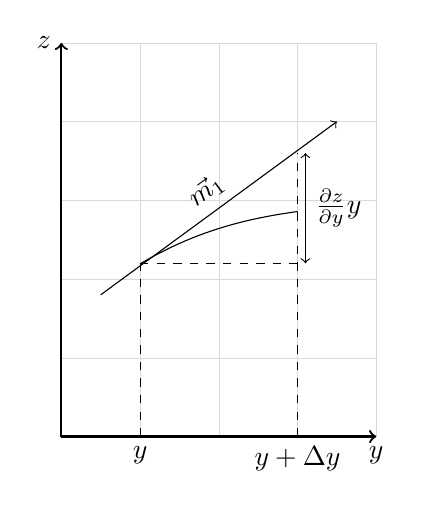
\begin{tikzpicture}
  \draw[very thin, gray!30, step = 1cm] (0, 0) grid (4, 5);
  \draw[domain = 1 : 3, variable = \x]
    plot ({\x}, {3 / (1 + e^(-\x))});

  \draw[thick] [->] (0, 0) -- (4, 0) node[right, below] {\(y\)};
  \draw[thick] [->] (0, 0) -- (0, 5) node[above, left] {\(z\)};

  \draw node[below] at (1, 0) {\(y\)};
  \draw node[below] at (3, 0) {\(y + \Delta y\)};

  \draw[dashed] (1, 0) -- (1, 2.2);
  \draw[dashed] (3, 0) -- (3, 3.6);

  \draw[dashed] (1, 2.2) -- (3, 2.2);
  \draw[<->] (3.1, 2.2) -- (3.1, 3.6)
    node[midway, right] {\(\frac{\partial z}{\partial y} \dd y\)};

  \draw[->] (0.5, 1.8) -- (3.5, 4)
    node[midway, above, sloped] {\(\vec{m_{1}}\)};
\end{tikzpicture}

    \caption{\(x = const\)}\label{fig:proj_x}

  \end{subfigure}
  \qquad
  \begin{subfigure}[b]{0.3\textwidth}

    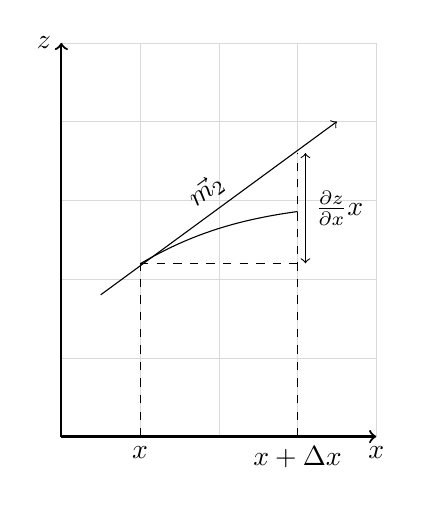
\begin{tikzpicture}
  \draw[very thin, gray!30, step = 1cm] (0, 0) grid (4, 5);
  \draw[domain = 1 : 3, variable = \x]
    plot ({\x}, {3 / (1 + e^(-\x))});

  \draw[thick] [->] (0, 0) -- (4, 0) node[right, below] {\(x\)};
  \draw[thick] [->] (0, 0) -- (0, 5) node[above, left] {\(z\)};

  \draw node[below] at (1, 0) {\(x\)};
  \draw node[below] at (3, 0) {\(x + \Delta x\)};

  \draw[dashed] (1, 0) -- (1, 2.2);
  \draw[dashed] (3, 0) -- (3, 3.6);

  \draw[dashed] (1, 2.2) -- (3, 2.2);
  \draw[<->] (3.1, 2.2) -- (3.1, 3.6)
    node[midway, right] {\(\frac{\partial z}{\partial x} \dd x\)};

  \draw[->] (0.5, 1.8) -- (3.5, 4)
    node[midway, above, sloped] {\(\vec{m_{2}}\)};
\end{tikzpicture}

    \caption{\(y = const\)}\label{fig:proj_y}

  \end{subfigure}
\end{figure}

\end{remark}

Проведем касательные \(\vec{m_{1}}\) и \(\vec{m_{2}}\) в плоскостях
\(x = const\) и \(y = const\). Их векторное произведение будет задавать нормаль
к поверхности в этой точке:
\(\vec{n} = \vec{m_{1}} \times \vec{m_{2}}\). Значит площадь
элементарного параллелограмма,построенного на \(m_{1}\) и \(m_{2}\), будет
\(\approx \dd \sigma\) с точностью до б.м. более высокого порядка.

Вычислим полученное векторное произведение:

\begin{align*}
  \vec{m_{1}} = (0, \dd y, \frac{\partial z}{\partial y} \dd y)
  \qquad
  \vec{m_{2}} = (\dd x, 0, \frac{\partial z}{\partial x} \dd x)
  \\
  \vec{n}
  = m_{1} \times m_{2}
  = \begin{vmatrix}
    \vec{i} & \vec{j} & \vec{k} \\
    0 & \dd y & \frac{\partial z}{\partial y} \dd y \\
    \dd x & 0 & \frac{\partial z}{\partial x} \dd x \\
  \end{vmatrix}
  =
  \underbrace{\left(
    \frac{\partial z}{\partial x},
    \frac{\partial z}{\partial y},
    -1
  \right)}_{\vec{p}} \dd x \dd y
\end{align*}

Нормируем и домножим на \(-1\) полученный вектор \(\vec{p}\), чтобы получить
единичный вектор  в направлении положительной нормали \(n_{0}^{+}\):

\begin{align*}
  n_{0}^{+}
  = \frac{(-z'_{x}, -z'_{y}, 1)}{\sqrt{1 + (z'_{x})^2 + (z'_{y})^2}}
  \implies \cos \gamma = \frac{1}{{\sqrt{1 + (z'_{x})^2 + (z'_{y})^2}}}
\end{align*}

Итак, площадь элементарного параллелограмма будет равна:

\begin{align*}
  \dd \sigma
  = \abs{\vec{n}}
  \approx \sqrt{1 + (z'_{x})^2 + (z'_{y})^2} \abs{\dd x \dd y}
  = \frac{1}{\abs{\cos \gamma}} \abs{\dd x \dd y}
  \implies \dd x \dd y \approx \pm \cos \gamma \dd \sigma
\end{align*}

Аналогично \(\dd x \dd z = \pm \cos \beta \dd \sigma\),
\(\dd y \dd z = \pm \cos \alpha \dd \sigma\).

\begin{remark}
  \(\dd \sigma > 0\) как площадь элементарного участка. \(\dd x \dd y\),
  \(\dd x \dd z\), \(\dd y \dd z\) это проекции \(\dd \sigma\) и их знак
  зависит от обхода \(\dd \sigma\), т.е. от знака нормали \(\vec{n}\). Далее
  опустим \(\pm\), т.к. косинус учитывает знак, т.е. при \(\dd x \dd y < 0\)
  будет \(\cos \gamma < 0\).
\end{remark}

Переведем полученную ранее формулу для поверхностного интеграла 2-ого рода в
координатную форму:

\begin{align*}\label{surf-int-coords}\tag{SIC}
  \iint_{S} (\vec{F} \cdot \vec{n_{0}}) \dd \sigma
  = \iint_{S} (P, Q, R) \cdot (\cos \alpha, \cos \beta, \cos \gamma) \dd \sigma
  = \iint_{S} (P \cos \alpha + Q \cos \beta + R \cos \gamma) \dd \sigma
\end{align*}

Подставим в это выражение полученные формулы связи \(\dd \sigma\) с
\(\dd x \dd y\), \(\dd x \dd z\) и \(\dd y \dd z\). Получим формулу для
поверхностного интеграла 2-ого рода в проекциях:

\begin{align*}\label{surf-int-proj}\tag{SIP}
  \iint_{S} P \dd y \dd z + Q \dd x \dd z + R \dd x \dd y
\end{align*}